\documentclass[11pt, letterpaper]{article}
\usepackage{graphicx}
\usepackage[a4paper, margin=4em, footskip=2em]{geometry}
\usepackage{parskip}

\title{
    Implementační dokumentace k 2. úloze do IPP 2023/2024 \\
    Jméno a příjmení: Michal Cenek \\
    Login: xcenek04
}
\date{}

\begin{document}

\maketitle

\section{Návrh}

Dle zadání je řešení ve třídě \texttt{Interpret}, které implementuje abstraktní třídu \texttt{AbstractInterpret}.
Přetížená metoda \texttt{parseXml} zpracuje vstupní XML soubor a vytvoří interní reprezentaci kódu.


Interní reprezentace kódu je tvořena seznamem objektů třídy \texttt{Instruction}. Každý objekt instrukce obsahuje operační kód, pořadí a seznam argumentů typu \texttt{Argument}. Třída argument obsahuje typ argumentu a jeho text.
Text má odstraněné bílé znaky na začátku a na konci escape sekvence jsou převedeny na odpovídající znaky.
Dál argument zatím není zpracován a je uložen jako řetězec.


Data která reprezentují stav interpretu jsou členy třídy \texttt{Interpret}. Obsahují dočasný rámec,
globální rámec, zásobník lokálních ramáců, zásobník volání, datový zásobník, čítač instrukcí a tabulku návěští.
Dále \texttt{Interpret} obsahuje pomocné metody, které jsou volány z metody \texttt{execute}.


Výjimky jsou ošetřeny vyvoláním výjimky tříd dědících ze třídy \texttt{IPPException}.
Kromě výjimek z rámce ipp core jsou implementoval třídy \texttt{InterpretRuntimeException} a \texttt{SourceStructureException}.
Třída \texttt{InterpretRuntimeException} je vyvolána při běhu interpretu při chybách 51 až 58.
Třída \texttt{SourceStructureException} je vyvolána při zpracování XML souboru s kódem 32.

\section{Implementace}

Metoda \texttt{execute} volá metody \texttt{getDOMDocument} z rámce ipp core a výsledek předává metodě \texttt{parseXml}.
Metoda \texttt{parseXml} zkontroluje správnost vstupního souboru a vytvoří interní reprezentaci kódu.
Vykonávání instrukcí je implementování pomocí čítače instrukcí, smyčky která běží dokud není čítač instrukcí na konci seznamu instrukcí nebo dokud nebyl program ukončen instrukcí EXIT nebo dokud nenastane sémantická chyba.
Uvnitř smyčky je posloupnost if - elseif příkazů, která podle operačního kódu provede příslušnou instrukci.
Při vykonávání instrukcí jsou použity pomocné metody třídy \texttt{Interpret}.
Metoda \texttt{selectFrame} vybere rámec podle jeho názvu.
Metoda \texttt{getSymbolValue} vrátí hodnotu proměnné nebo literálu.
\texttt{setVariable} nastaví hodnotu proměnné ve správném datovém rámci.
Metoda \texttt{unescape} převede escape sekvence na odpovídající znaky.
\texttt{parseLiteral} zpracuje literál a vrátí jeho hodnotu.
\texttt{getFrame} vrátí rámec podle jeho názvu.
Metoda \texttt{getVariableName} vrátí název proměnné bez rámce a znaku @.

\begin{figure}[h]
  \centering
  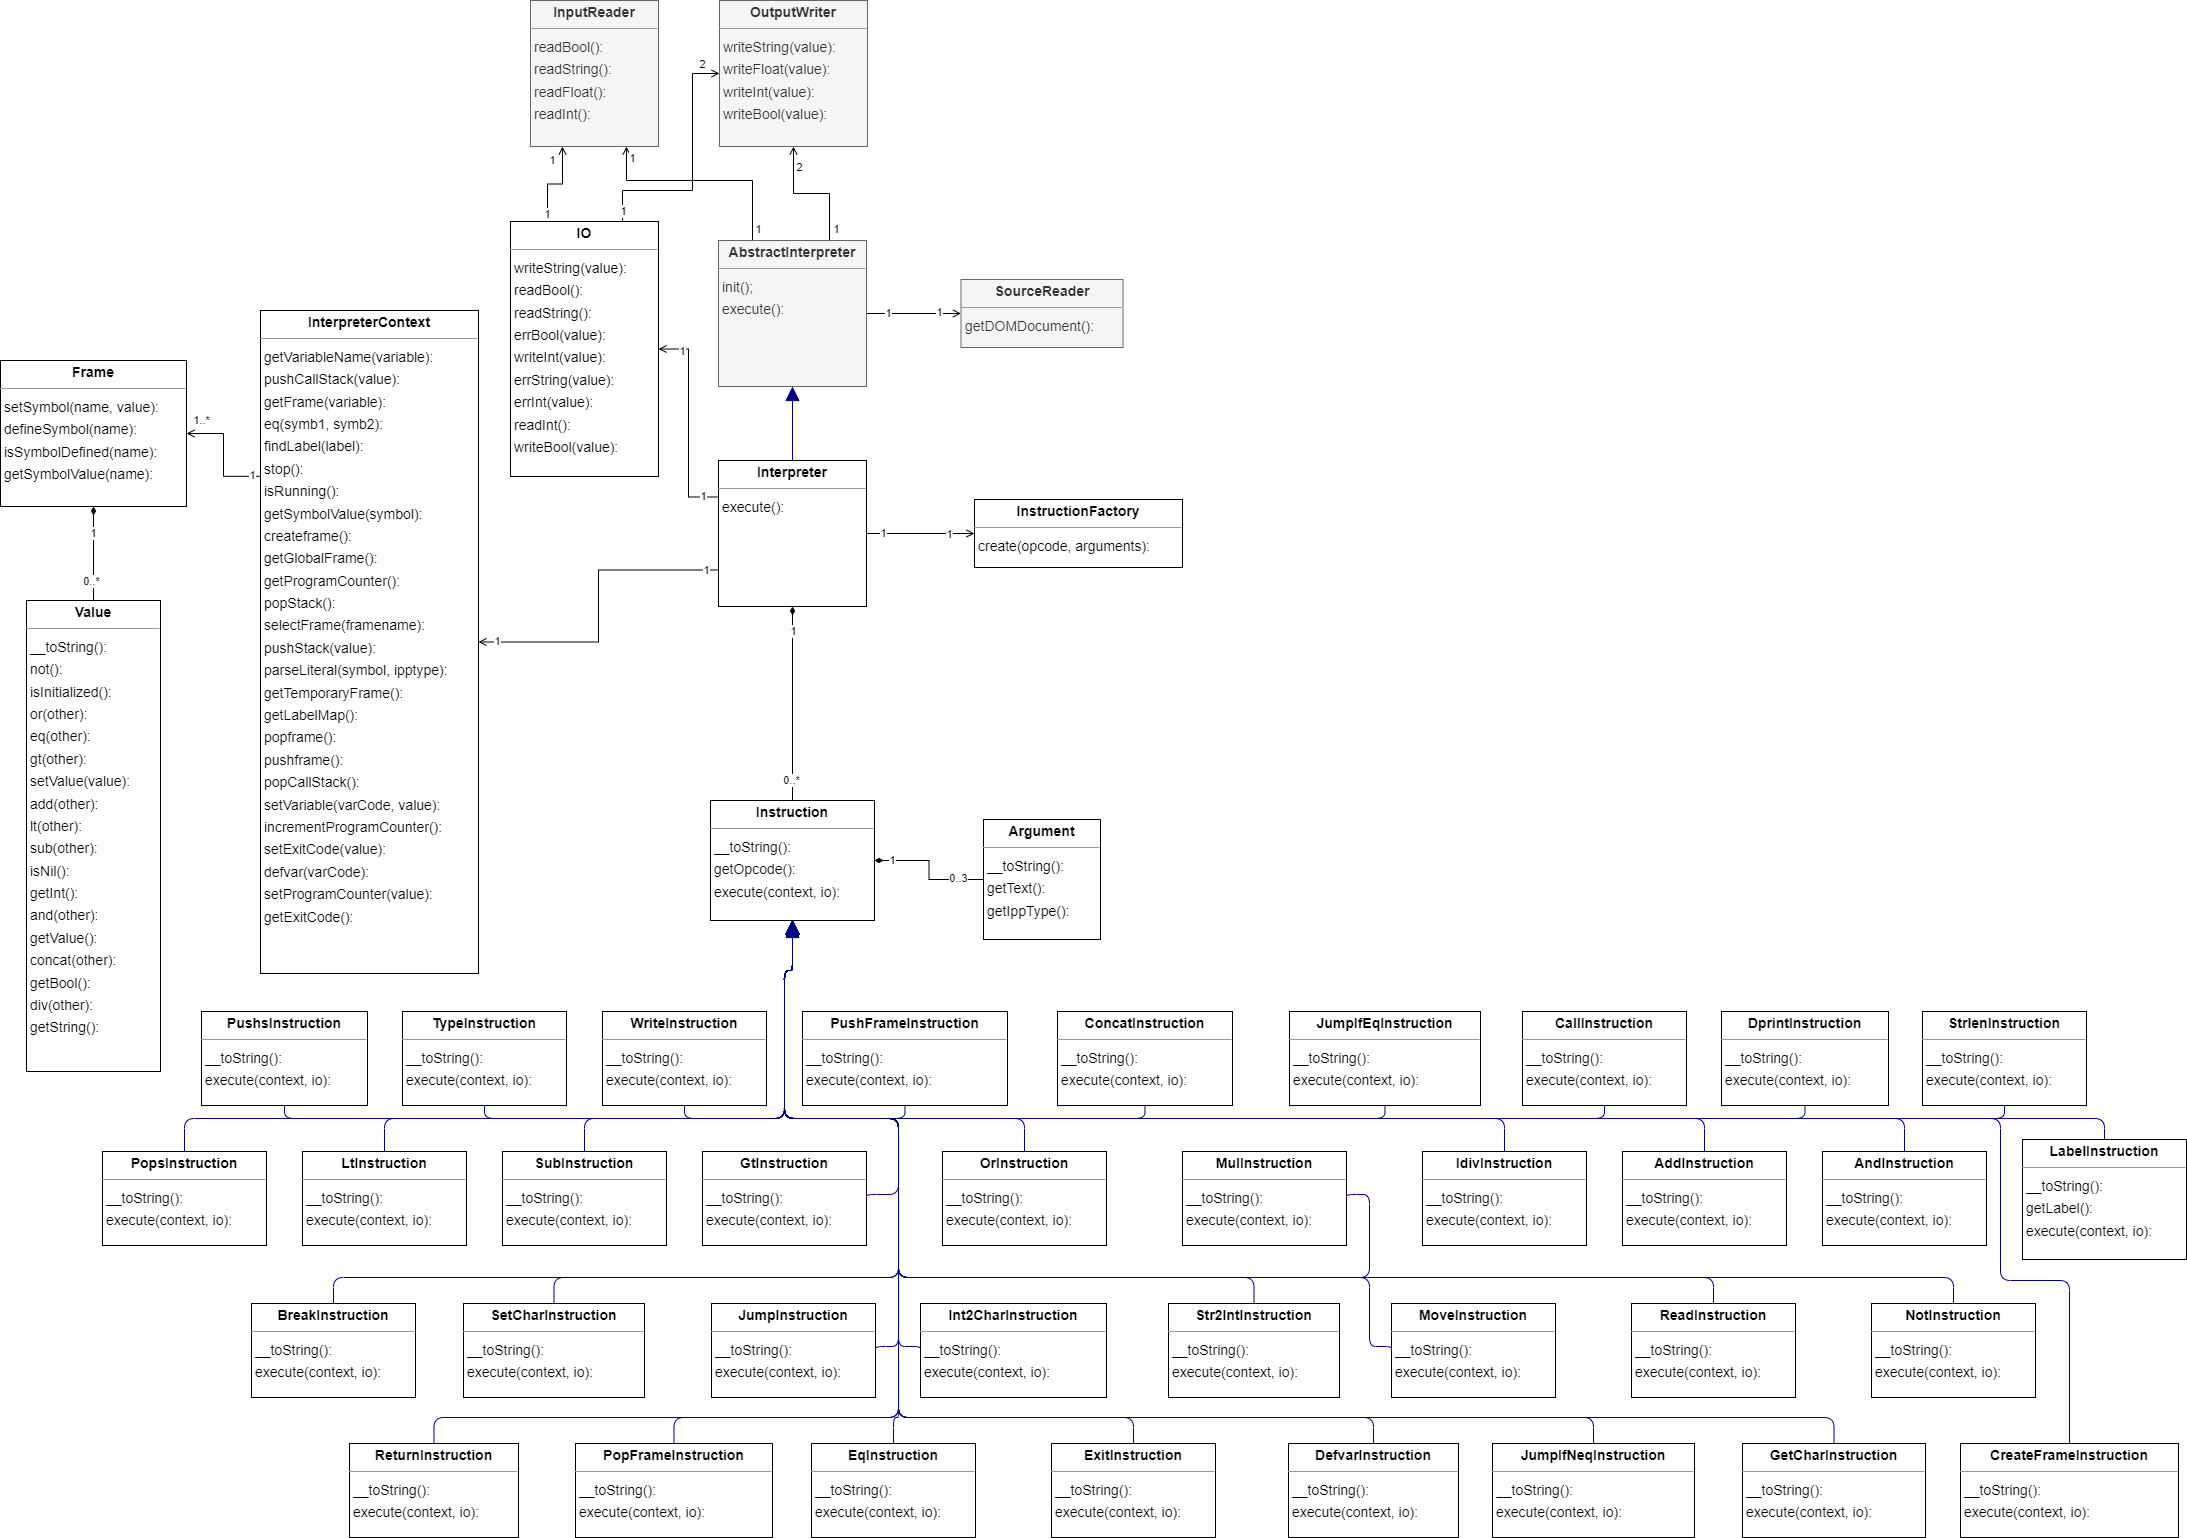
\includegraphics[width=0.75\textwidth]{diagram.png}
  \caption{Diagram tříd.}
  \label{fig:diagram}
\end{figure}

\end{document}
